% Hazi Feladat / Meresi jegyzokony sablon BME MIT
% Keszult: 2012.13.17
% Leiras: Ebbe a fajlba kerul a lenyegi resz, a szoveg. A legfelsobb szintu felsorolas a section (chapter nem hasznalatos).

\section{A mérés bemutatása}


\section{Otthoni feladat 1}
\subsection{Leírás}
A laborsegédlet és az egyéb segédanyagok maradéktalan elolvasását és megértését követően
töltse le a labor weblapjáról ( http://www.mit.bme.hu/oktatas/targyak/vimim223/feladat/5-Szavazas-es-aukcio ) a
labor forráskódjait, és bontsa ki a forráskódokat a  msclab01 könyvtárba. Ezt
követően indítson el Eclipse alól egy JADE platform-ot, majd legalább három
msclab01.votingauction\_lab.VoterAgent.VoterAgent szavazó ágenst (pl.  va0 ,
va1 , és  va2 néven) a voting01.cfg szavazási
konfigurációnak megfelelő – akár egyező, akár különböző – jelöltekkel, illetve egy
msclab01.votingauction\_lab.VotingMechanismAgent.VotingMechanismAgent
szavazásvezérlő ágenst (pl.  vma néven) az előbb említett konfigurációval.
\begin{enumerate}
	\item Figyelje meg és értelmezze a működést.
	\item Kövesse nyomon Sniffer ágenssel az ágensek közti üzenetcserét.
	\item Mit tapasztal?
	\item Más-más szavazó ágens paraméterek megadása hatására hogy viselkedik a rendszer?
	\item Milyen szabályok szerint zajlik a szavazás?
	\item Mi az előnye, és mi a hátulütője ennek a fajtájú szavazásnak?
	\item A lefutás során/után milyen adatok jöttek létre a log
	könyvtárban?
\end{enumerate}
\subsection{Megoldás}
Futattam az ágenseket a következő run config-ot használva:
\begin{lstlisting}[caption=Szavazás run config, frame=single,float=!ht]
-container  -port  1099  -host  localhost
AAAAAA:msclab01.votingauction\_lab.VoterAgent.VoterAgent(mathias)
BBBBBB:msclab01.votingauction\_lab.VoterAgent.VoterAgent(mandela)
CCCCCC:msclab01.votingauction\_lab.VoterAgent.VoterAgent(mandela)
DDDDDD:msclab01.votingauction\_lab.VoterAgent.VoterAgent(valakimas) vma:msclab01.votingauction_lab.VotingMechanismAgent.VotingMechanismAgent(cfg\backslash voting01.cfg)
\end{lstlisting}
\begin{figure}[!h]
\begin{center}
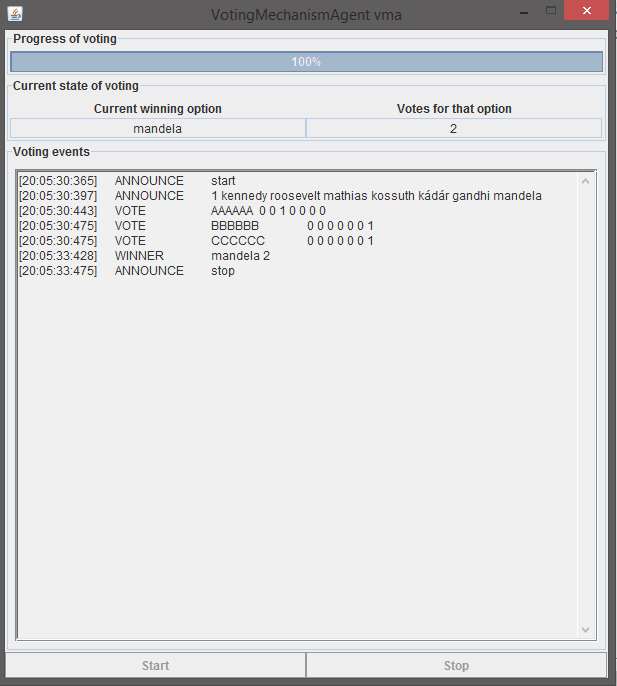
\includegraphics[height=7cm]{figures/ofel1a1.png}
\caption{A szavazás eredménye}
\end{center}
\end{figure}
\begin{figure}[!h]
\begin{center}
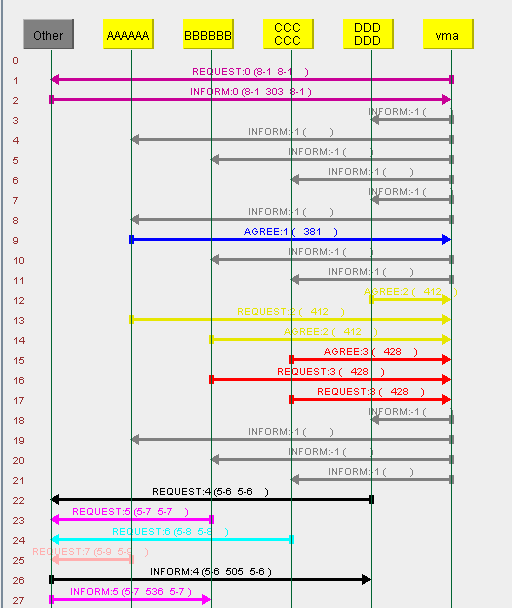
\includegraphics[height=7cm]{figures/ofel1a2.png}
\caption{Az ágensek közötti komunikáció}
\end{center}
\end{figure}
\begin{lstlisting}[caption=A log.txt tartalma, frame=single,float=!ht]
[20:16:23:533]	ANNOUNCE	start
[20:16:23:549]	ANNOUNCE	1 kennedy roosevelt mathias kossuth kádár gandhi mandela
[20:16:23:565]	VOTE		BBBBBB	0 0 0 0 0 0 1
[20:16:23:565]	VOTE		AAAAAA	0 0 1 0 0 0 0
[20:16:23:580]	VOTE		CCCCCC	0 0 0 0 0 0 1
[20:16:26:596]	WINNER	mandela 2
[20:16:26:596]	ANNOUNCE	stop
\end{lstlisting}
\begin{lstlisting}[caption=A rest.txt tartalma, frame=single,float=!ht]
Name	Won
----	---
DDDDDD	no
BBBBBB	yes
AAAAAA	no
CCCCCC	yes
\end{lstlisting}

Az implementált szavazás egyfordulós többségi szavazás. Ennek a szavazásnak az a hátránya hogy a kisebbség döntheti el a kimenetelét. Tegyük fel hogy 2-en akarják az A jelöltet, és egy-egy szavazó akarja a B,C,D jelöltet, de semmiképp az A-t. Ebben az esetben a kisebbség akarata érvényespül és az A nyer.

\section{Otthoni feladat 2}
\subsection{Leírás}
Tegye több (legalább két) körös runoff szavazássá az előbbi protokollt! Ehhez
megfelelőképp írja át a  VotingMechanismAgent szavazásvezérlő ágens  maxRounds
változóját, majd tesztelje az előbbi feladathoz hasonlóan a rendszert.  Megjegyzés:
többkörös szimpla többségi runoff szavazás esetén, ha a szavazás egy adott körében nem születik
egyértelmű végeredmény, azaz nincs egy opció, amely a beérkezett szavazatok alapján maximális
minősítésű, úgy a több maximális minősítésű opcióval újabb szavazás kerül kiírásra.
\subsection{Megoldás}
\begin{figure}[!h]
\begin{center}
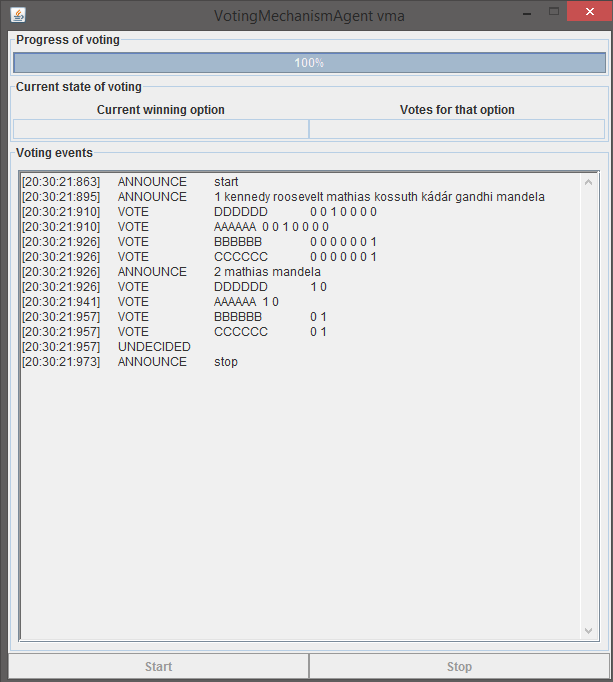
\includegraphics[height=7cm]{figures/ofel2.png}
\caption{Többfordulós szavazás}
\end{center}
\end{figure}
A feladatnak megfelelően, módosítottam a VotingMechanismAgent-et, így döntetlen esetén egy újabb forduló lesz a két jelölt között.

\section{Otthoni feladat 3}
\subsection{Leírás}
Alakítsa át a szavazást többségi elven működő szavazássá (majority rule voting)!
Ehhez  egészítse  ki  a  VotingMechanismAgent ágens  AnnounceAndWait
viselkedésének  action() metódusában, a  case 1 részben (mikor  state=1 , azaz az
ágens  szavazatokra  vár)  a  megfelelő  két  feltételvizsgálatot
( if(CommonMethods.maxNum(votes) == 1) ) úgy, hogy ne csak azt nézzék, hogy
egyetlen maximális minősítésű opció van-e az eddig beérkezett szavazatok alapján,
hanem azt is, hogy a szavazatok száma erre az opcióra legalább az ágensek számának
fele-e, vagy sem. Tesztelje a módosított szavazási protokollt az előbbi feladatokhoz
hasonlóan, és foglalja össze, ill. magyarázza meg a különbségeket és hasonlóságokat!
\subsection{Megoldás}

\begin{figure}[!h]
\begin{center}
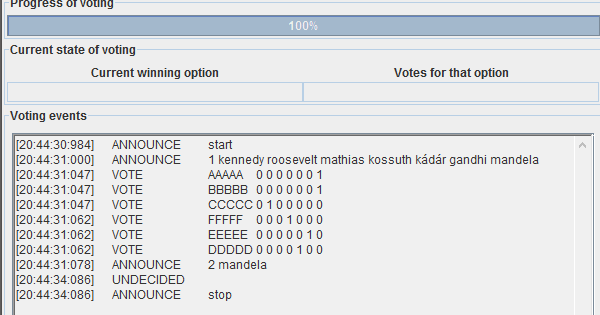
\includegraphics[height=7cm]{figures/ofel3_1.png}
\caption{Minősített többségi szavazás döntetlen}
\end{center}
\end{figure}
\begin{figure}[!h]
\begin{center}
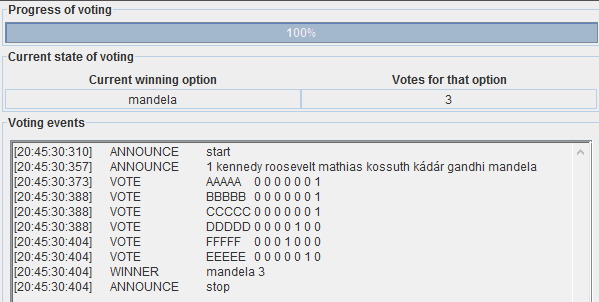
\includegraphics[height=7cm]{figures/ofel3_2.png}
\caption{Minősített többségi szavazás győztessel}
\end{center}
\end{figure}
A mínősített többségi elven működő szavazás elkerüli az egyszerű többségi szavazás hibáját, hogy a kisebbség dönt. Hátránya hogy több jelölt esetén valószínütlen, hogy egy jelölt eléri az 50%+1 szavazatot, így ez a szavazási módszer nem hírdet győztest.

\section{Otthoni feladat 4}
\subsection{Leírás}
Térjünk  most  át  az  aukciókra!  Indítson  el  legalább  három
msclab01.votingauction_lab.BidderAgent.BidderAgent licitáló ágenst (pl.  ba0 ,
ba1 , és  ba2 néven) a  auction01.cfg aukció
konfigurációval,  illetve  egy
msclab01.votingauction\_lab.AuctioneerAgent.AuctioneerAgent árverező
ágenst is (pl.  aa néven) ugyanezzel.
\begin{enumerate}
	\item Figyelje meg és értelmezze a működést.
	\item Kövesse nyomon Sniffer ágenssel az ágensek közti üzenetcserét.
	\item Mit tapasztal?
	\item Milyen szabályok szerint zajlik az aukció?
	\item Mi az előnye, és mi a hátulütője ennek a fajtájú aukciónak?
	\item A lefutás során/után milyen adatok jöttek létre a log
	könyvtárban?
	\item Milyen licitálási stratégia szerint játszik most a BidderAgent ágens?
	\item Szorgalmi feladat: próbáljon meg javítani a BidderAgent ágens licitálási stratégiáján, és
	magyarázza meg, hogy mit és miért csinált!
\end{enumerate}
\subsection{Megoldás}
\end{figure}
\begin{figure}[!h]
\begin{center}
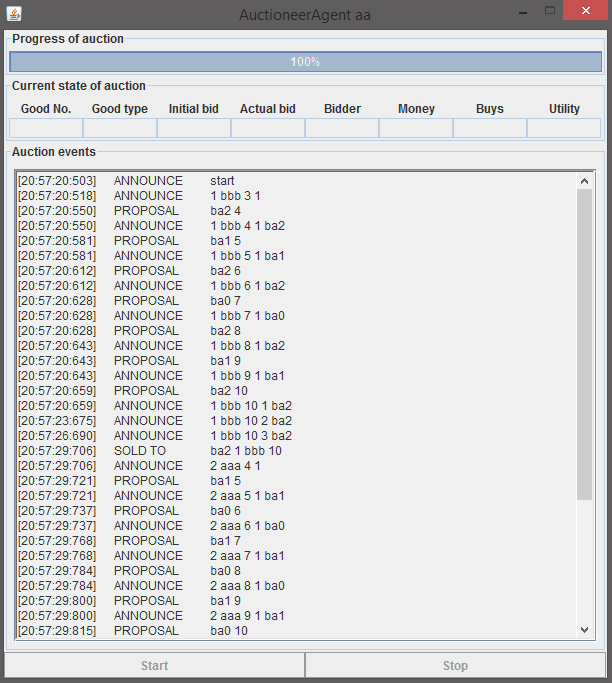
\includegraphics[height=7cm]{figures/ofel4.png}
\caption{Minősített többségi szavazás}
\end{center}
\end{figure}
Az aukción az kapja meg a terméket, aki a legtöbbet adja érte. Három leütés is implementálva van, de az ágensek egyszerű stratégiája és gyorsasága miatt nem történik változás a leütések alatt. Amint a kimenetből is látható, az ágensek mindenképpen meg akarják venni a termékeket, emelve a licitet ha nem ők adták rá a legnagyobbat. Így amikor egy ágens végül elnyeri a terméket és csökkenti a rendelkezésére álló pénzt, a többi termék esetén már nem képes eljutni a maximális liciting. Az aukció végén így minden ágens 1 terméket vásárolt meg, legjobban az utolsó ágens járt, hisz neki már nem volt versenytársa, a többi ágens maximális áron vásároltak.

\section{Labor feladat 1}
\subsection{Leírás}
Alakítsa át a VoterAgent szavazó ágenst úgy, hogy ne csak egy, hanem több opcióra is
képes legyen egy-egy körben szavazni (ehhez akár a VotingMechanismAgent ágens
szavazási konfigurációjához hasonló konfigurációt is létrehozhat számára, vagy átadhatja a
több óhajtott opciót bemeneti paraméterként, ha egyszerűbb, vagy lehet akár véletlenszerű is,
hogy mire szavaz az ágens)! Ehhez a ParticipateInVoting viselkedés case 1 esetét
kell módosítani. Ennek kapcsán ne felejtse el kivenni a VotingMechanismAgent ágens
AnnounceAndWait viselkedésének action() metódusában a case 1 rész for
ciklusából a break-et. Tesztelje a működést! Mit tapasztal? Hogyan zajlik ez az újfajta,
úgynevezett engedélyező szavazás (approval voting)? Mi a különbség, hasonlóság, előny,
hátrány az előzőleg megvalósított/kipróbált módszerekhez képest?
\subsection{Megoldás}
\begin{lstlisting}[caption=Engedélyező run-config, frame=single,float=!ht]
AAAAA:msclab01.votingauction_lab.VoterAgent.VoterAgent_1(mandela,gandhi)
BBBBB:msclab01.votingauction_lab.VoterAgent.VoterAgent_1(mandela)
CCCCC:msclab01.votingauction_lab.VoterAgent.VoterAgent_1(kennedy,gandhi,mandela)
vma:msclab01.votingauction_lab.VotingMechanismAgent.VotingMechanismAgent(voting01.cfg)
\end{lstlisting}
Az ágensek paraméterei azok a jelöltek, akiket engedélyeznek. Ennek a szavazásmódnak az előnye, hogy nincs szükség több fordulóra, hiszen a szavazók megadják az összes olyan jelöltet akit elfogadnának. Hátránya hogy nem tudjuk hogy az elfogadott jelöltek között milyen sorrend van.
\begin{figure}[!h]
\begin{center}
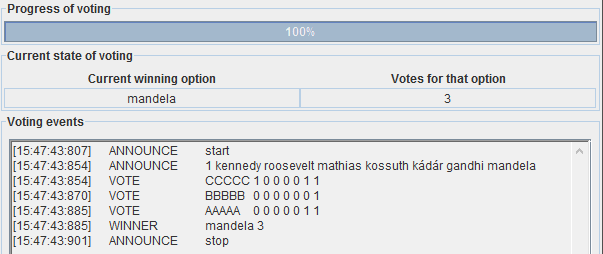
\includegraphics[height=7cm]{figures/fel1.png}
\caption{Engedélyező szavazás}
\end{center}
\end{figure}

\section{Labor feladat 2}
\subsection{Leírás}
Az előbbiekhez hasonlóan módosítsa most a VoterAgent szavazó ágenst úgy, hogy adott
határok közt pontozni is tudja az egyes opciókat (ne csak binárisan szavazzon)! Tesztelje az
így létrejött újfajta, úgynevezett pontozó szavazást (rated voting)! Mi a különbség,
hasonlóság, előny, hátrány az előző módszerekhez képest?
\subsection{Megoldás}
\begin{lstlisting}[caption=Pontozó run-config, frame=single,float=!ht]
AAAAA:msclab01.votingauction_lab.VoterAgent.VoterAgent_2(mandela:-1,gandhi:10)
BBBBB:msclab01.votingauction_lab.VoterAgent.VoterAgent_2(mandela:5)
CCCCC:msclab01.votingauction_lab.VoterAgent.VoterAgent_2(kennedy:4,gandhi:-2,mandela:3)
vma:msclab01.votingauction_lab.VotingMechanismAgent.VotingMechanismAgent(voting01.cfg)
\end{lstlisting}
Mint látható az ágenseknek megadjuk, hogy melyik jelöltnek milyen pontot adjanak. Azon jelöltek akik nem szerepelnek, 0 pontot kapnak. A szavazatok összeszámolása nem változik az előbbihez képest. A szavazás ezen formája már rögzít egy preferenciasorrendet a jelöltek között, ami az engedélyező szavazásnál nem volt jelen. A hátránya az hogy a szavazók szélsőséges pontokat adva a jelölteknek, az összegzésnél elnyomják a többi szavazó pontozását.
\begin{figure}[!h]
\begin{center}
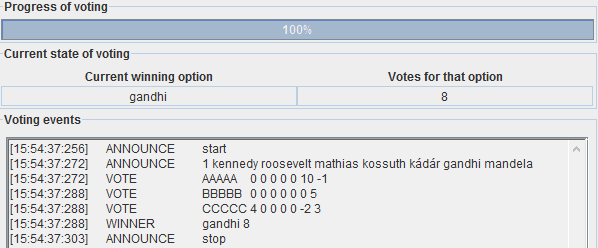
\includegraphics[height=7cm]{figures/fel2.png}
\caption{Pontozó szavazás}
\end{center}
\end{figure}

\section{Labor feladat 3}
\subsection{Leírás}
Az előbbiekhez hasonlóan módosítsa most még tovább a VoterAgent szavazó ágenst úgy,
hogy már rangsorolni is tudja az opciókat (0-tól (k-1)-ig, ha k darab opció van)! Tesztelje az
így létrejött újfajta, úgynevezett Borda-féle rangsor alapú számlálást (Borda count)! Mi a
különbség, hasonlóság, előny, hátrány az előzőekhez képest?
\subsection{Megoldás}
\begin{lstlisting}[caption=Használt run-config, frame=single,float=!ht]
AAAAA:msclab01.votingauction_lab.VoterAgent.VoterAgent_3(mandela,gandhi)
BBBBB:msclab01.votingauction_lab.VoterAgent.VoterAgent_3(mandela)
CCCCC:msclab01.votingauction_lab.VoterAgent.VoterAgent_3(kennedy,gandhi,mandela)
vma:msclab01.votingauction_lab.VotingMechanismAgent.VotingMechanismAgent(voting01.cfg)
\end{lstlisting}
Az ágensek újra egy preferencia-sorrendet kapnak, az első jelölt fogja kapni a legnagyobb súlyt, az utána következő 1-el kissebbet és így tovább. A fel nem sorolt jelöltek 0 pontot kapnak. A legnagyobb súly egyenlő a jelöltek számával, amit az ágens a VotingMechanismAgent-től kap meg. Hasonlít a pontozó szavazásra, a különbség a pontok halmaza, ami itt 0-tól N-ig, ahol  N a jelöltek száma. Érzékeny az irreleváns alternatíva elhagyására. Ez azt jelenti hogy ha elhagyjuk azt a jelöltet aki a legkevesebb pontot kapta és újra számoljuk a pontokat, akkor nem biztos hogy az eredeti győztes lesz az új győztes.
\begin{figure}[!h]
\begin{center}
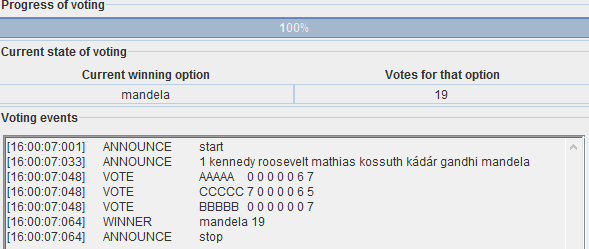
\includegraphics[height=7cm]{figures/fel3.png}
\caption{Borda szavazás}
\end{center}
\end{figure}

\section{Labor feladat 4}
\subsection{Leírás}
Most pedig térjünk át az aukciókra! Hozzon létre japán aukciót! Ehhez például átírhatja a
BidderAgent licitáló ágensek licitálási stratégiáját úgy, hogy egy adott összeg fölött
„szálljanak ki az aukcióból”, azaz ne növeljék tovább a mások által megemelt tétet, de még
szebb megoldás, ha külön üzenetváltást vezetünk be erre a célra a BidderAgent licitáló
ágensek, és az AuctioneerAgent árverező ágens között. Pl. a licitáló küldhet egy
DISAGREE performatívájú üzenetet az árverezőnek („kimehet a szobából”), mire az árverező
kiveheti őt az aukcióból, és ezt a többi/maradék licitálónak is a tudomására hozhatja pl. egy
megfelelő INFORM üzenetben. Teszteljük, és értelmezzük a működést! Helyesen zajlik az
aukció? Jobb-e, vagy rosszabb, mint az előző? Miért?
\subsection{Megoldás}
\begin{lstlisting}[caption=Használt run-config, frame=single,float=!ht]
ba0:msclab01.votingauction_lab.BidderAgent.JapBidderAgent(auction01.cfg)
ba1:msclab01.votingauction_lab.BidderAgent.JapBidderAgent(auction01.cfg)
ba2:msclab01.votingauction_lab.BidderAgent.JapBidderAgent(auction01.cfg)
aa:msclab01.votingauction_lab.AuctioneerAgent.JapAuctioneerAgent(auction01.cfg)
\end{lstlisting}
A megoldásom két új üzenet bevezetéséből áll, a REJECT\_PROPOSAL és az INFORM(won). Az elsőt egy licitáló ágens akkor küldi, ha számára az adott termék jelenlegi licitje túl nagy és ki szeretne szállni az aukcióból. Az aukcióvezető ágens fordulónként növeli a licitet és fogadja az időközben érkező REJECT\_PROPOSAL üzeneteket. Mikor csak 1 ágens maradt az aukcióban, akkor a vezető neki elküld egy INFORM(won) üzenetet, értesítvén hogy ő nyerte meg a terméket. Az ágensek egyszerű stratégiával rendelkeznek, ha a jelenlegi licit nagyobb mint a maximális ár - random(3), akkor az ágens kilép a licitációból.
\begin{figure}[!h]
\begin{center}
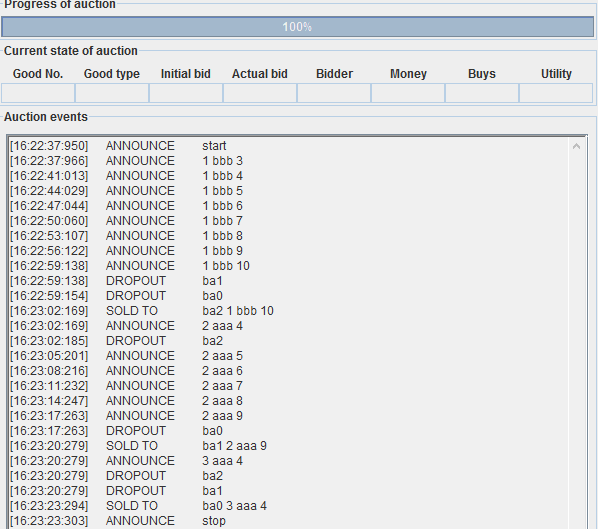
\includegraphics[height=7cm]{figures/fel4.png}
\caption{Japán aukció}
\end{center}
\end{figure}

\section{Labor feladat 5}
\subsection{Leírás}
Alakítsa át az előbbi aukciót holland aukcióvá! Ehhez írja át az AuctioneerAgent
árverező ágens AnnounceAndWait viselkedésének action() metódusa case 1 esetét
(úgy, hogy licit esetén azonnal menjünk át state=2-be!), illetve írjuk át megfelelőképp a
„kalapács leütéséért” felelős TimeoutHandler osztály onWake() metódusát is
(tájékozódjunk a bő kommentek alapján). Érdemes felfigyelnünk az aukció végét jelző
harmadik leütésre, mikor az if(round == 3) feltételvizsgálat teljesül. Ez a
feltételvizsgálat a holland aukció esetén nyilván inkább valami olyasmi kellene, hogy legyen,
ami azt vizsgálja, hogy egy-egy termék kapcsán egy adott minimális ár alá mentünk-e már,
vagy sem. Ha igen, akkor vége az aukciónak (hiszen a termék nem kelt el még a minimális
áron sem), egyébként nincs vége. Azt is gondoljuk meg, hogy a BidderAgent ágensek
részéről érkező licitek ekkor már nem az árverező által megajánlott összeg fölött kellene, hogy
legyenek, hanem azzal egyenértékűek. Viszont ezt nyilván az AuctioneerAgent árverező
ágensnél is át kell vezetni (proposal == bid)… Ha elkészültünk, teszteljük, és
értelmezzük a működést! Helyesen zajlik az aukció? Jobb/rosszabb, mint az előzőek? Miért?
\subsection{Megoldás}
\begin{lstlisting}[caption=Használt run-config, frame=single,float=!ht]
ba0:msclab01.votingauction_lab.BidderAgent.HolBidderAgent(auction01.cfg)
ba1:msclab01.votingauction_lab.BidderAgent.HolBidderAgent(auction01.cfg)
ba2:msclab01.votingauction_lab.BidderAgent.HolBidderAgent(auction01.cfg)
aa:msclab01.votingauction_lab.AuctioneerAgent.HolAuctioneerAgent(auction01.cfg)
\end{lstlisting}
\begin{figure}[!h]
\begin{center}
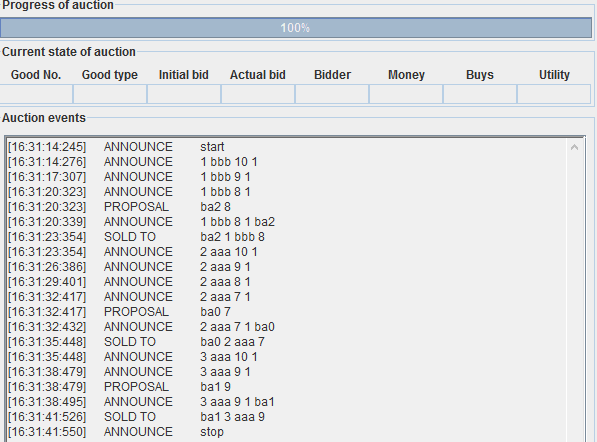
\includegraphics[height=7cm]{figures/fel5.png}
\caption{Japán aukció}
\end{center}
\end{figure}
Az ágensek itt csak akkor licitálnak, ha az aktuális licit <= sajátpénz - rand.nextInt(4). Az aukcióvezető vár licitekre, de ha nem kap akkor 1-el csökkenti az aktuális licitet. A kezdeti licit a maximális ár és ha az aktuális licit a minimális ár alá csökken, akkor a vezető nem eladottnak tekinti a terméket.


\section{Összefoglalás}
